\documentclass[twoside]{uva-inf-bachelor-thesis}
\usepackage[english]{babel}
\usepackage{outlines}

\usepackage{amsmath}
\usepackage{textcomp}
\usepackage{csquotes}
\usepackage{biblatex}
\usepackage{braket}
\usepackage{graphicx}
\usepackage{xspace}
\usepackage{tikz}
\usetikzlibrary{positioning}

\addbibresource{refs.bib}

\usepackage{fontspec}
%\setmainfont[Ligatures={Common,TeX}]{Adobe Caslon Pro}
%\setsansfont{Source Sans Pro}
%\setmonofont{Iosevka}
\usepackage{listings}

\lstset{language=[ARM]Assembler,numbers=left,basicstyle=\small\ttfamily}

\newcommand{\code}[1]{\lstinline[breaklines=true]{#1}}
\newcommand{\ucosiii}{\textmu C/OS-III\xspace}
\newcommand{\ucosii}{\textmu C/OS-II\xspace}
\newcommand{\ucpu}{\textmu C/CPU\xspace}
\newcommand{\ucos}{\textmu C/OS\xspace}
\newcommand{\task}[1]{\ensuremath{\tau_#1}}

\usepackage{booktabs}

\makeatletter
\define@key{Gin}{resolution}{\pdfimageresolution=#1\relax}
\makeatother

\title{Predictable, guarantee-based\\ scheduling in the \ucosiii\\ real-time operating system}
\author{Sam van Kampen}
\supervisors{T. Walstra}
\signedby{Signees}


\begin{document}

\maketitle

\begin{abstract}
    In this thesis, the performance and utility of Earliest Deadline First scheduling in combination with the processor demand guarantee criterion is evaluated in the \ucosiii real-time operating system on a first-generation Raspberry Pi, and contrasted with \ucosiii's default, priority-based scheduler.
\end{abstract}


\tableofcontents

%
%
% I N T R O D U C T I O N
%
%

\chapter{Introduction}
In our day-to-day computing, we are usually not concerned with predictability when it comes to program execution time. If running a program takes slightly longer than it does normally, or our system becomes temporarily unresponsive, we may be annoyed, but no disastrous consequences are induced. In other systems, however, the consequences of irregular execution times can be dangerous or even fatal. A computing system that must react within precise time constraints to environmental events is called a (hard)\footnote{Sometimes, a distinction is made between hard real-time systems and soft real-time systems. In soft real-time systems, the consequences of missing time constraints are not catastrophic, but merely lead to `degraded system performance'. The distinction between soft real-time and non-real-time tasks is often blurry, however, since there is almost always a soft deadline by which we want a task to produce results. The value of the soft real-time paradigm mostly seems to be in optimizing the value gained from executing tasks where value varies between tasks. The topic of soft real-time computing is not discussed further in this thesis, so whenever the term `real-time' is used, it can be read to refer to hard real-time systems.} real-time system\cite{buttazzo2011hard}. In these systems, correct behavior depends on the results of computations but also the time at which they are produced. Examples can mostly be found in the embedded market, ranging from industrial automation or military equipment to traffic control systems.

Due to the focus of real-time systems on executing actions within a given time frame, these systems are often said to have to be \textit{fast}. This framing is, however, misleading. When we talk about speed, what do we mean? In a real-time scenario, a system is required to provide a guarantee that tasks can be successfully executed within the given time constraints. In order to do this, the system needs to be \textit{fast enough} to react to its environment, but it also needs to have a high degree of predictability. Features of modern computing systems that speed up average response time (and would, therefore, make a real-time system `faster' by some definition of `fast') are therefore often eschewed in favor of predictability: examples include demand paging or `cycle-stealing' implementations of \textit{Direct Memory Access} (DMA).

To implement a real-time computing system, the entire system can be written from the ground up, without using any existing code. This can often be costly in terms of time, however. In order to facilitate quick development of real-time systems, `general-purpose' real-time operating systems have been developed, which contain facilities like task management, mutual exclusion primitives, et cetera.

\subsubsection{\ucos} \label{sec:ucos}
The real-time operating system that is used in this thesis is called \textit{\ucosiii}. The original version of \ucos was written in 1991 by Jean J. Labrosse, due to dissatisfaction with commercial kernel offerings at the time. As the decade came to a close, Labrosse decided to work on the operating system full-time, founding Micrium, Inc., which currently develops and sells the kernel commercially, with source available at no cost for research purposes. Versions of \ucos have been used in a wide variety of applications, among them NASA's Curiosity Rover\footnote{https://www.micrium.com/about/customer-stories/curiosity/}. It is especially suited to this thesis because of the breadth of its documentation: firstly, an extensive manual \cite{micrium:ucosmanual} is supplied with the source code, and secondly, the source code itself is heavily commented and written with readability in mind.

\subsubsection{Research question}
As described above, predictability is a vital part of real-time systems. Naturally, in systems that consist of multiple tasks, an important factor in guaranteeing task execution within given deadlines is the \textit{task scheduler}. As noted in \textcite{buttazzo2011hard}, however, many real-time kernels lack functionality that guarantees task execution. In many cases, a general priority-based scheduler is implemented, with possible round-robin scheduling functionality. Therefore, in this thesis, I will explore the benefits of guarantee-based scheduling algorithms through both literature analysis and through the implementation of a guarantee-based scheduling algorithm in a real-time operating system (\ucosiii), and by evaluating it on real hardware (a first-generation Raspberry Pi). The research question I am aiming to answer is:

\begin{outline}
    \itemsep=0em
    \1 What is the performance and usability effect of implementing a guarantee-based scheduling algorithm in a real-time operating system, as compared to the commonly implemented priority-based scheduling algorithm?
\end{outline}


\subsubsection{Data availability}
All data and code used in the production of this thesis is available online, with instructions on how to run the experiments on real hardware, at \url{https://github.com/svkampen/thesis}.



%
%
% R E L A T E D  W O R K
%
%

\chapter{Related work}
Running \ucos on the Raspberry Pi has been explored earlier, most notably in a thesis by \textcite{sfd:realpi}, which details the porting of \ucosii to a number of different versions of the Pi. The port in this work differs, both in the operating system version used and the hardware used on the Pi, most notably when it comes to the choice of UART and timer.

On the topic of scheduling in \ucos specifically, not much research seems to have been done - perhaps due to its lack of open-source licensing. Nevertheless, there is some interesting work in this area.

\textcite{tue:hfs} describe a two-level hierarchical scheduling framework, which allows system designers to partition system tasks into subsystems which have their own scheduling budget and strategy. The framework is subsequently implemented and evaluated on hardware running \ucosii. 

\textcite{Cho2011} define a scheduling algorithm for \ucosii which mixes its default priority-based scheduler with Earliest Deadline First in a best-effort configuration, and uses deadline misses as a metric to perform dynamic voltage and frequency scaling (DVFS).

\textcite{dodiu2010} adapt \ucosii scheduling to be interrupt-priority-aware, in the sense that tasks are given interrupt masks which are switched out on context switch. This way, high-priority tasks are not interrupted by an interrupt associated with a lower-priority task.

When it comes to scheduling more generally, there is a breadth of research to explore.
Historically important papers in the field include Liu and Layland's seminal 1973 paper\cite{Liu1973}, which describes the Earliest Deadline First algorithm, and \textcite{Lehoczky1989}, which analyzes the Rate Monotonic scheduling algorithm.

\textcite{salmani2005modified} describe the Modified Maximum Urgency First scheduling algorithm, which improves upon the Earliest Deadline First algorithm used in this thesis by improving transient overload handling. A version of this algorithm adapted for distributed real-time systems is discussed in \textcite{chen2006flexible}, and extensions to the algorithm are explored in \textcite{behera2012enhanced}.

%
%
% S C H E D U L I N G
%
%

\chapter{Scheduling}
In contemporary operating systems, it is common to have many programs in memory, executing concurrently. This concept is called \textit{multitasking}. To give the illusion of multiple programs running `at the same time' on a single core, program execution is interleaved, by letting a program run for a small time slice before switching to another. The criteria that are used to assign tasks to the CPU are contained in a \textit{scheduling policy}. 

\section{The scheduling problem}
\textcite{buttazzo2011hard} defines the scheduling problem as follows. Given a set of $n$ tasks $\Gamma = \set{\tau_1, \tau_2, \ldots, \tau_n}$, a set of $m$ processors $P = \set{P_1, P_2, \ldots, P_m}$, a set of $s$ types of resources $R = \set{R_1, R_2, \ldots, R_s}$, a directed acyclic graph (DAG) describing the precedence relation among tasks, and a set of timing constraints associated with each task, assign processors from $P$ and resources from $R$ to tasks in $\Gamma$ in order to complete all tasks under the specified constraints. The scheduling problem, in its general form, has been shown to be NP-complete, and hence computationally intractable.

Despite this general intractability, many algorithms have been developed which solve a more specific version of the scheduling problem. These scheduling algorithms have some common characteristics, which are outlined below.

\section{Characteristics of scheduling algorithms}
The following scheduling algorithm classes are adapted from \textcite{buttazzo2011hard}:
\begin{outline}
    \1 Preemptive vs. Non-preemptive
        \2 In preemptive schedulers, a running task can be interrupted at any time and switched out for another task.
        \2 In non-preemptive algorithms, a task is executed until completion.
    \1 Static vs. Dynamic
        \2 In static schedulers, scheduling decisions are taken based on parameters that do not change as the system is running. In dynamic schedulers, these parameters can change during system evolution.
    \1 Guarantee-based vs. Best-effort
        \2 In a guarantee-based scheduling algorithm, tasks are only accepted if a guarantee can be made that they can be scheduled, whereas in a best-effort system, tasks may be accepted that cannot be allowed to run to completion for fear of jeopardizing other tasks.
\end{outline}

\section{Task characteristics in real-time systems}
Scheduling algorithms usually make decisions on which task to schedule based on characteristics of the tasks in the given task set, perhaps augmented with characteristics of the system they are running on. A few task characteristics that are common on real-time systems, and used in the scheduling algorithms below, are detailed below.

\begin{outline}
    \1 A task's \textbf{arrival time} ($a_i$) (also called \textbf{release time} $r_i$) is the time at which a task becomes ready for execution;
    \1 A task's \textbf{computation time} ($C_i$) is the time necessary for the processor to execute the task, without interruption;
    \1 A task's \textbf{absolute deadline} ($d_i$) is the time before which a task should be completed to avoid damage to the system;
    \1 A task's \textbf{relative deadline} ($D_i$) is the difference between the task's arrival time and its absolute deadline: $D_i = d_i - a_i$;
    \1 A task's \textbf{finishing time} ($f_i$) is the time at which a task finishes execution;
    \1 A task's \textbf{lateness} ($L_i$) is the difference between the task's absolute deadline and its finishing time.
\end{outline}

An illustration of these characteristics can be seen in figure~\ref{fig:taskcharacteristics}.

\begin{figure}[htpb]
    \centering
    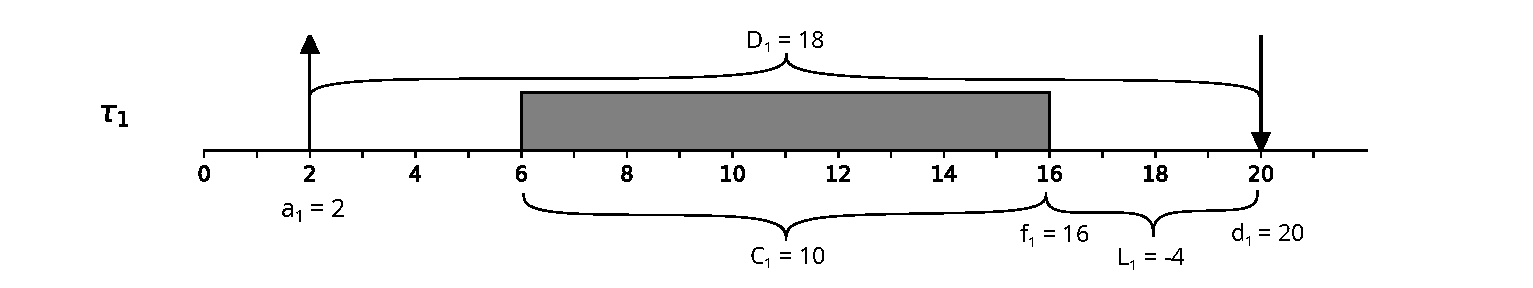
\includegraphics[width=\textwidth]{taskcharacteristics.eps}
    \caption{An overview of common real-time task characteristics.}
    \label{fig:taskcharacteristics}
\end{figure}

\section{Static scheduling algorithms}
As mentioned in the list of scheduling algorithm characteristics, \emph{static scheduling algorithms} do not take varying system behavior into account, and make use of characteristics that are known at system start. 

\subsection{Rate Monotonic}
\emph{Rate Monotonic} is a scheduling algorithm for periodic task sets which assigns priorities based on the frequency of the task. Id est, if the task needs to run more often, it gets a higher priority.Rate Monotonic is a fixed-priority assignment, so task priorities do not change over time. \textcite{Liu1973} proved the optimality of Rate Monotonic among fixed-priority assignments.

One issue when using Rate Monotonic-based scheduling is its low upper bound on processor utilization; As the number of tasks $n$ tends to infinity, the maximum processor utilization which will yield a valid RM schedule tends to $\ln 2 \approx 0.69$.

\section{Dynamic scheduling algorithms}

\subsection{Earliest Deadline First}
The \emph{Earliest Deadline First} algorithm is an elegant solution to the problem of scheduling $n$ independent tasks on a uniprocessor system, with dynamic arrivals and preemption. The algorithm simply picks the task with the earliest absolute deadline among all ready tasks, and executes it. When a new task arrives with an earlier deadline, the running task is preempted in favor of the new task.

\subsubsection{Guarantees}
There are multiple ways of giving guarantees based on an EDF schedule, depending on the characteristics of the task sets, such as periodicity, synchronicity of arrival times and synchronicity of relative deadline and period. The guarantee criterion implemented in this work is based on the processor demand criterion as outlined in \textcite{Baruah1990}.

\subsubsection{Precedence constraints}
Using a transformation on the task set, EDF can be extended to handle dependent tasks\cite{Chetto1990}. The idea is as follows. Say we have a task set, with two tasks: \task{1} and \task{2}, where \task{2} is dependent on \task{1}. To honor this precedence constraint, we can modify the arrival time of \task{2}, so that it cannot start before \task{1} has finished. Note that, if there is a valid schedule for the task set which satisfies the precedence constraint, the following conditions are met:

\begin{align}
    s_2 \ge a_2 \quad &\text{(\task{2} cannot start before its arrival time)}\\
    s_2 \ge a_1 + C_1 \quad &\text{(\task{2} cannot start before the minimum finishing time of \task{1})}
\end{align}

To guarantee both of these, we can set $s_2$ equal to $\max(a_2, a_1 + C_1)$.

Similarly, task deadlines need to be modified, so that \task{1} finishes before the last possible start time of \task{2}, that being $d_2 - C_2$.

\section{Combining periodic and aperiodic tasks}
One characteristic of the scheduling algorithms that have been discussed in the previous sections is whether they can be used with periodic or aperiodic tasks, or both. In all cases, however, we have looked at homogeneous task sets - that is, task sets that either consist purely of periodic, or purely of aperiodic task sets. In this section, algorithms that can handle heterogeneous task sets are discussed.

The idea behind many of these algorithms is to compute the processor utilization of the periodic task set, and set aside the rest of the processor utilization to be used by a so-called \emph{task server}, which handles aperiodic requests. The processor utilization set aside for the server, denoted $U_s$, is often called the \emph{bandwidth} of the server.

\subsection{Background Scheduling}
The simplest way of scheduling aperiodic tasks is through \emph{Background Scheduling} - simply running them when the system would otherwise be idle. One obvious downside is the large possible aperiodic task response time; periodic tasks which could be postponed while still meeting their deadlines are instead run earlier than they have to be.

\subsection{Total Bandwidth Server}
The \emph{Total Bandwidth Server} is a server for aperiodic jobs which is used in conjunction with the EDF algorithm. When an aperiodic job $j_k$ enters the system, at $t = a_k$, it receives a deadline

\[ d_k = \max(a_k, d_{k-1}) + \frac{C_k}{U_s} \]

where $U_s$ is the server bandwidth and $C_k$ is the job's worst-case execution time. The name of the server is reflected in the fact that the total bandwidth over a given time period is given to the job.

After this deadline is assigned, the job is scheduled by the EDF algorithm, as are the periodic tasks in the system.

\subsubsection{Optimizing TBS: deadline advancement}
Note that this deadline is pessimistic, in the sense that it could be set earlier, improving aperiodic response time, if the finishing time of $j_k$, $f_k$, is earlier than its assigned deadline. This can occur depending on when periodic tasks are scheduled, since the deadline accounts for the worst-case finishing time given the processor utilization used by periodic tasks. For instance, let us take the situation in figure~\ref{fig:tbsworstdeadline}. Here, we have periodic processor utilization $U_p = \frac{5}{6}$, and server bandwidth $U_s = \frac{1}{6}$. The deadline assigned to $j_k$, which has computation time $C_k = 2$ and arrives at $t = 2$, is therefore $d_k = 2 + \frac{C_k}{U_s} = 14$. Due to the strange (non-EDF) periodic schedule, it also finishes at $t = 14$. EDF, with deadline $d_k = 14$, produces a schedule where $j_k$ finishes at $f_k = 12$ (fig. \ref{fig:tbsedfdeadline}). Knowing this, we could set its deadline to $12$. However, if we then recompute its EDF schedule, we will find that the task finishes even earlier. This process can be repeated to find $j_k$'s earliest finishing time, $f^*_k$, which turns out to be $5$, as can be seen in figure~\ref{fig:tbsoptimaldeadline}. As you can see, the response time of $j_k$ can be greatly improved, without jeopardizing periodic tasks. This does, however, add computational complexity, due to the fact that evaluating $f^*_k$ requires (repeatedly) computing the EDF schedule up to the finishing time of $j_k$.

\begin{figure}[htpb]
    \centering
    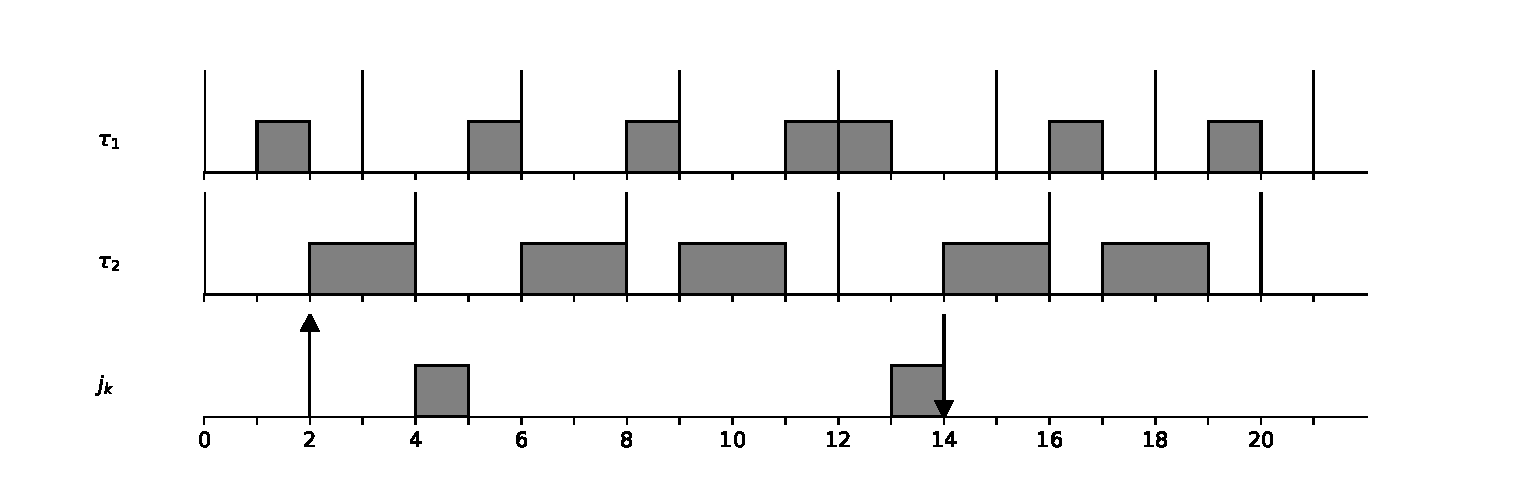
\includegraphics[width=0.85\textwidth]{worstcasedeadline.eps}
    \caption{A situation where job $j_k$ finishes exactly at its deadline.}
    \label{fig:tbsworstdeadline}
\end{figure}

\begin{figure}[htpb]
    \centering
    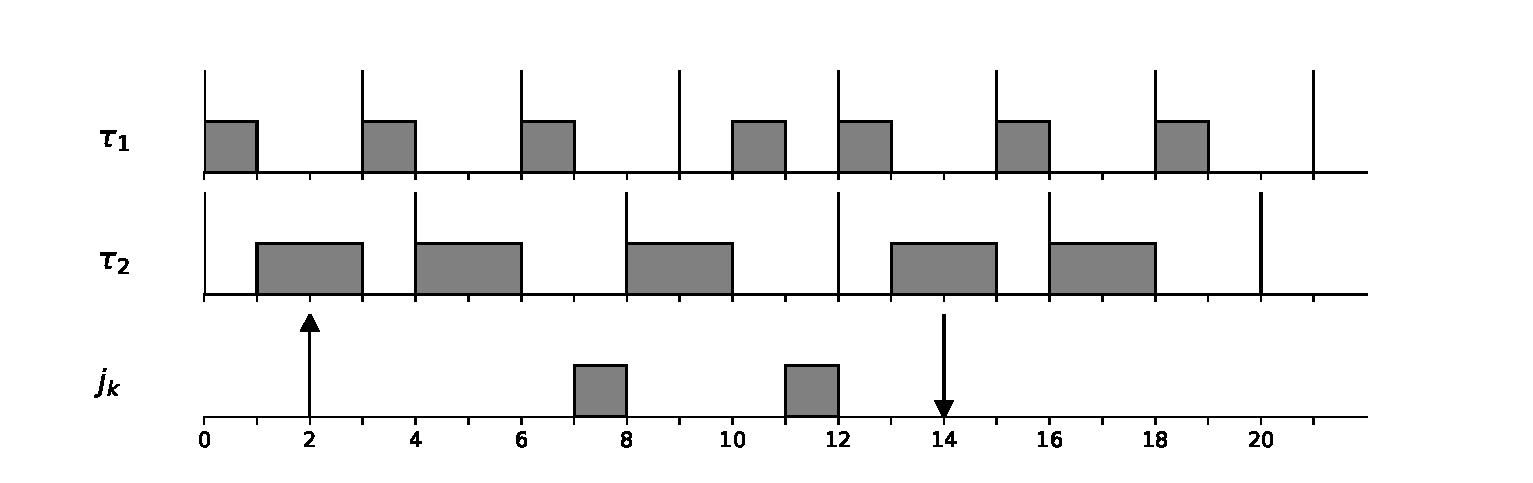
\includegraphics[width=0.85\textwidth]{edfdeadline.eps}
    \caption{The situation produced by EDF, where $f_k$ = 12.}
    \label{fig:tbsedfdeadline}
\end{figure}

\begin{figure}[htpb]
    \centering
    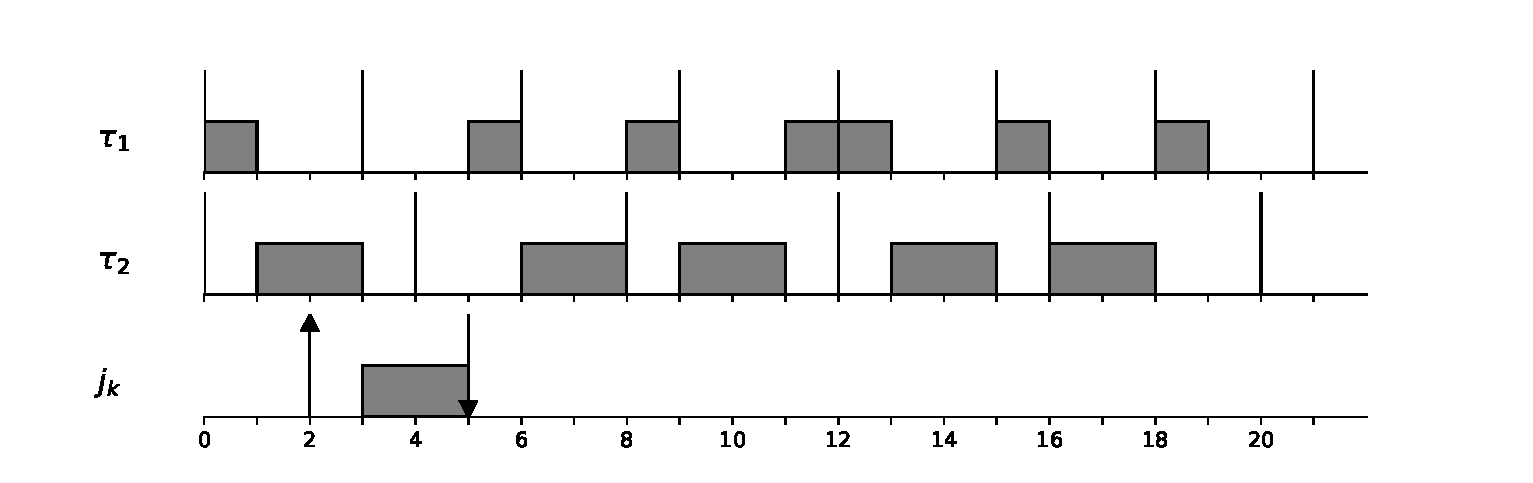
\includegraphics[width=0.8\textwidth]{optimaldeadline.eps}
    \caption{The situation where $j_k$ finishes at the earliest possible time.}
    \label{fig:tbsoptimaldeadline}
\end{figure}

\section{Scheduling in \ucosiii}
Just as in many real-time operating systems, the scheduler used in \ucosiii is a generic priority-based scheduler. In these schedulers, tasks are assigned priorities and the scheduler simply runs the highest priority ready task. The priorities are assigned at task creation, but there is optional support for changing priorities at run-time. The number of priority levels is configurable at compile time.

There is optional support for round-robin scheduling. If it is enabled and multiple tasks are ready at a given priority level, in a cyclical fashion, each task is run for a time quantum, which is configurable at task creation time.

The flexibility in the number of priority levels seems to suggest that many dynamic scheduling algorithms (such as EDF) could be built on top of this priority-based scheduler. Every additional priority level, however, brings a memory cost with it. \ucos uses a \textit{priority bitmap} (see fig.~\ref{fig:priobitmap}) to keep track of which priorities have associated ready tasks, and each priority has its own ready list. This diminishes the flexibility of the scheduler, but improves the scheduling performance in the case where the number of priorities is fairly low.

\section{Worst-case Execution Time Analysis}
One of the task parameters which is essential when guarantee-based scheduling is applied is the worst-case execution time of a task. The worst-case execution time needs to be accurately determined, as an underestimation can induce invalid guarantees. Additionally, a pessimistic worst-case execution time will cause the system to reject task sets which may have been feasible in practice. This raises the question: how can worst-case execution times be accurately determined?

Worst-case execution time analysis is a whole discipline unto itself, with a range of analytical and measurement-based approaches. Ideally, a mix of analytical and measurement-based approaches is used, as analytical static analysis often fails to take into account run-time behavior such as caching, while a purely measurement-based approach may be limited due to the rare occurrence of extremely long execution times.

\textcite{hansen_et_al:wcet} detail a method of determining worst-case execution times based on a fusion of measurement-based and analytical approaches. The method makes use of Extreme Value Theory (EVT), a branch of mathematics which is concerned with reasoning about the tail end of distributions. Using EVT, the paper posits that the so-called \emph{block maxima} of execution times are distributed according to the Generalized Extreme Value distribution\footnote{A similar concept which the reader may be familiar with is the Central Limit Theorem, which states that, under certain conditions, sample means are normally distributed.}, and the parameters of that distribution can be fit to sample data. Using the distribution, a probabilistic worst-case execution time can then be determined, along with a probability that the execution time is exceeded.

\begin{figure}[htpb]
    \centering
    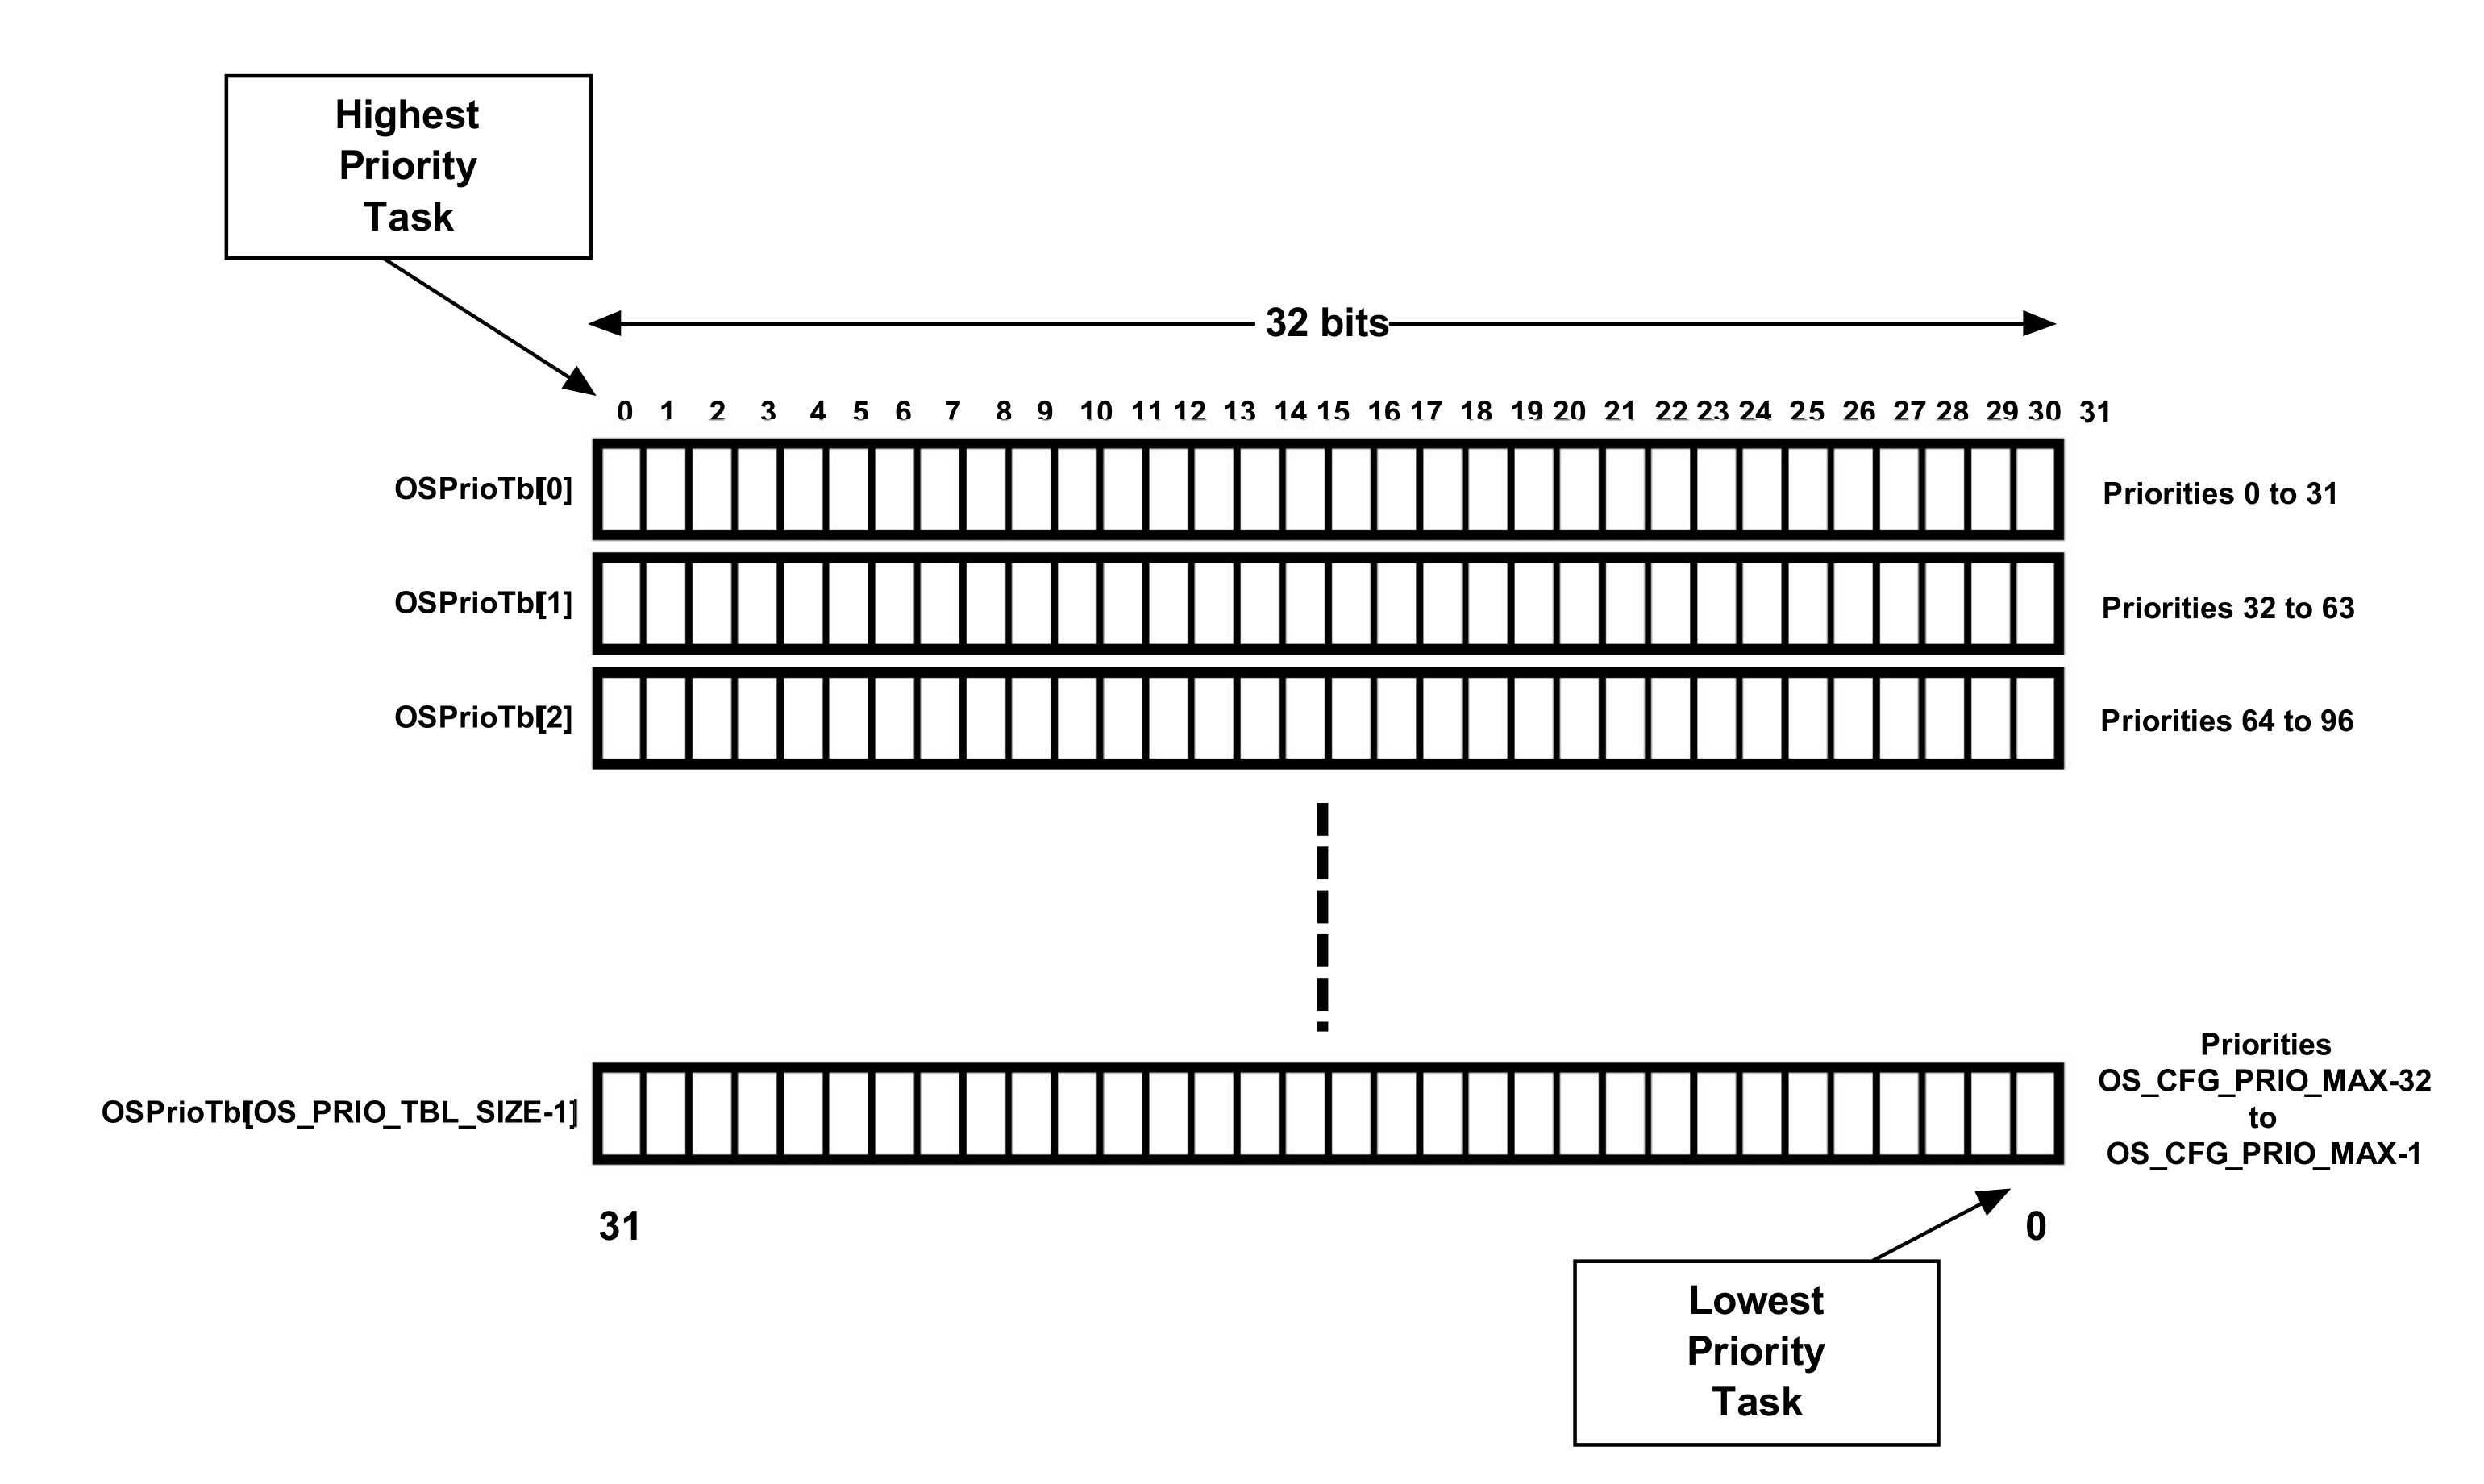
\includegraphics[width=0.8\textwidth]{priobitmap.png}
    \caption{An illustration of \ucosiii's priority bitmap. Taken from the user manual, figure 6-3. If a bit is set, it indicates a ready task in the ready list of the associated priority. The highest priority task can be found quickly by using processors' `count-leading-zeros' instruction.}
    \label{fig:priobitmap}
\end{figure}

%\subsection{The scheduling implementation}

%
%
% H A R D W A R E
%
%

\chapter{Hardware} \label{chp:hardware}
Real-time operating systems run on a broad range of hardware. Running tests on all of this different hardware is, of course, impossible. For this thesis, I have chosen to use a piece of hardware which exemplifies a number of characteristics of real-time systems, but which is also readily available and well-documented: a first-generation Raspberry Pi.

\section{The Raspberry Pi 1B}
The hardware used in this thesis is a Raspberry Pi 1B, a single-board computer from early 2012. While it was marketed as an educational `toy' for children to learn how to program on, it became popular mainly as a cheap development board for (hardware) hobbyists, due to its ability to control electronics using its general purpose I/O (GPIO) pins, and its low price point of \$25-35 (depending on model). Its hardware is as follows:

\begin{outline}
    \1 A Broadcom BCM2835 System-on-Chip, including:
        \2 A single-core 700MHz ARM11 (ARMv6) processor
        \2 A VideoCore IV graphics processor
        \2 512 megabytes of RAM
    \1 26-pin General Purpose I/O (GPIO) header, capable of performing various functions
        \2 Serial I/O, SPI, software-controlled reading and writing at 3.3V
    \1 Ethernet, USB, HDMI and composite out, et cetera.
\end{outline}

The Pi has a number of desirable characteristics that make it suitable for use in this thesis. Firstly, it uses a low-power ARM processor, an architecture which is very common in embedded systems (with a market share of 37\% at the end of 2014 \cite{arm:embeddedmarketshare}). Additionally, its GPIO pins and their support for serial I/O allow for a simple way of interacting with the Raspberry Pi without having to implement USB or ethernet drivers. Such serial connections are also very common in embedded systems. Lastly, due to the popularity of the Pi, it is fairly well-documented. The datasheet that describes the hardware in the Raspberry Pi and how to interface with it is freely available\cite{bcm:2835peripherals}, and although it is occasionally inaccurate, there is a thorough list of errata available online\cite{bcm:2835errata}. Where the datasheet has omissions, there is also often information available online.

\subsection{General Purpose I/O}
As described above, the Raspberry Pi has 26 general purpose I/O pins. Some of these pins have a fixed function, but many have multiple functions, and which one a pin uses can be controlled by software. An overview of the 26-pin header and the functions of its pins can be seen in figure~\ref{fig:gpiopinout}. One thing of note is the fact that the pin numbering used on the header is not the same as is used in the BCM2835 peripherals manual; for instance, pin 7 on the header is GPIO pin 4 in the data sheet.

\begin{figure}[ht]
    \centering
    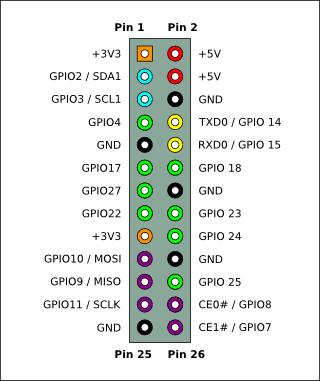
\includegraphics[scale=0.5]{Pi-GPIO-header-26-sm.png}
    \caption{The Raspberry Pi 1B GPIO pinout. Pins labeled \textit{GPIO \#} correspond to GPIO pins in the Broadcom BCM2835 peripherals manual\cite{bcm:2835peripherals}.}
    \label{fig:gpiopinout}
\end{figure}

\subsection{The VideoCore IV processor}
Coming from the x86 world, you might expect the VideoCore IV (VC4) GPU to be little more than a standard PC graphics card, managing and accelerating graphical output. While it does perform those actions, the VC4 has much broader responsibilities on the Raspberry Pi. It runs a (real-time) operating system of its own, ThreadX\cite{rpi:opensourcevpu}, and handles system initialization and the early boot process\cite{rpi:bootforum}. It also performs power and clock management\cite{rpi:gpuclockpower}. The way the clock management functions is however conveniently absent from the BCM2835 datasheet.

%
%
% P O R T I N G
%
%

\chapter{Porting \ucosiii to the Raspberry Pi}
To run \ucosiii on the Raspberry Pi, the operating system needs to be adapted to run on the hardware the Pi uses. These adaptations are commonly called \textit{ports}. There are ports to architectures that are similar to that of the Pi, such as the ARM9-based NXP LPC2923 \cite{micrium:nxplpc}, but there is no port for the Broadcom BCM2835, the SoC used by the Pi. This work includes such a port.

\section{The structure of \ucosiii}
The majority of \ucosiii is written as processor-independent C code, and can therefore be re-used in the port verbatim. Fragments of the operating system whose implementation is highly dependent on the target hardware, such as task switching or interaction with hardware timers, are implemented in separate source files. There is a CPU-specific component, \ucpu, which specifies CPU features such as the availability of a count-leading-zeros instruction, endianness, the size of data types such as timestamps, addresses, et cetera. Separately, OS-specific components such as task switching functions are defined. Lastly, a `Board Support Package' is defined, which contains the functionality that interacts with the on-board components such as the hardware timer and handles interrupts.

Of particular interest to the scheduler are the timer and the interrupt handling code.

\subsection{Timers}
In real-time systems, there obviously needs to be a correspondence between the time as measured in the system and external time. This is where hardware timers come in. The Raspberry Pi provides both running counter functionality (which allows the system to have a clock -- though it is not a real-time clock, which would keep an accurate date and time of day across reboots) and timer functionality (so the system is interrupted after a given time is elapsed).

As described in the BCM2835 peripheral data sheet, the Raspberry Pi contains two timers; a timer for the ARM processor itself and a system timer. Although \textcite{sfd:realpi} opts to use the ARM timer, the peripheral data sheet suggests using the system timer when accurate timing is required.\cite[p. 196]{bcm:2835peripherals}.

The system timer has microsecond resolution\footnote{Although the ARM timer has a higher frequency, it is not useful to us as the time taken to switch between tasks is already in the microsecond range.}, and consists of a 64-bit running counter and four 32-bit timer channels. These timer channels have a corresponding match register, which contains a 32-bit value that is compared with the running counter, triggering an interrupt when the lowest 32 bits of the running counter match the register value.

Two of the timer channels are in use by the VideoCore IV GPU, and are therefore not usable. Timer channel 1 and 3 are, however, available. We only need a single timer channel, and currently use timer channel 1.

\subsection{Interrupts}
As discussed in the previous section, the hardware timer can trigger an interrupt when a timer channel is matched. The system timer is one of the hardware components which is poorly described in the peripheral data sheet, but information found online can close that gap.

Interrupt handling in the ARM architecture differs significantly from similar features in the x86 architecture. Where the latter uses an interrupt vector table which dispatches a specific interrupt to a specific interrupt service routine, the former uses a much more generic approach.

ARM uses the term `exception' to mean an event which causes the processor to stop execution and jump to a piece of code to handle it. The ARM architecture supports seven kinds of exceptions: \textit{Reset}, \textit{Undefined Instruction}, \textit{Software Interrupt}, \textit{Prefetch Abort}, \textit{Data Abort}, \textit{Interrupt} (IRQ) and \textit{Fast Interrupt} (FIQ). When an exception is generated, the CPU jumps to an \textit{exception vector} for the given exception. These vectors are usually located at the beginning of the address space, but can be remapped. An overview of exception types, their corresponding processor mode and address that execution starts at after exception reception is given in table~\ref{tbl:exceptions}.

\begin{table}[h]
    \centering
    \begin{tabular}{lll}
        \toprule
        \textbf{Exception type} & \textbf{Processor mode} & \textbf{Execution address} \\
        \midrule
        Reset & Supervisor & \texttt{0x00000000} \\
        Undefined instructions & Undefined & \texttt{0x00000004} \\
        Software interrupt & Supervisor & \texttt{0x00000008} \\
        Prefetch Abort & Abort & \texttt{0x0000000C} \\
        Data Abort & Abort & \texttt{0x00000010} \\
        IRQ (interrupt) & IRQ & \texttt{0x00000018} \\
        FIQ (fast interrupt) & FIQ & \texttt{0x0000001C} \\
        \bottomrule
    \end{tabular}
    \caption{An overview of ARM exceptions. Adapted from table A2-4 in the ARM Architecture Reference Manual\cite{arm:arm}.}
    \label{tbl:exceptions}
\end{table}

In effect, processor faults and software interrupts have their own exception, and all `normal' device interrupts are coalesced into the `interrupt' and `fast interrupt' exceptions. The exception handling code, then, is tasked with determining which device caused the interrupt. The means of determining the interrupting device differ, as they often rely on hardware-provided memory-mapped registers. This is no different on the Raspberry Pi -- the peripheral data sheet details the interrupt mechanism in some detail on page 109. The peripheral data sheet however fails to mention the interrupt number assigned to the system timer. Some sleuthing reveals that the system timer channels are mapped at the start of the interrupt numbers, so IRQ 0 refers to the first timer channel, IRQ 1 to the second, et cetera.

As mentioned, the interrupts are handled either by the `fast interrupt' handler or the normal `interrupt' handler. The BCM2835 allows the systems programmer to route a single interrupt source to the fast interrupt vector, which has more banked registers and therefore allows for faster interrupt processing. This is not used in the port currently, as it would complicate the task switching code, which can currently use the same assembly for returning to voluntarily yielded code and interrupted code.

\subsection{Serial I/O} \label{sec:miniuart}
Implementing input/output capabilities is not strictly required to get \ucosiii running on the Raspberry Pi. An operating system is of little use without any I/O capabilities, however, and being able to output debugging information is also of great use in porting.

The type of I/O that the port has support for is very common in embedded devices, and was used throughout much of the twentieth century for communication between computers and associated terminals: serial communication using a UART. The peripheral data sheet tells us that the Raspberry Pi contains two UARTs, a primary ARM PL011 UART and a secondary so-called `mini UART'. Due to limitations such as the shallow FIFOs, this port uses the primary UART.

On the hardware side, the UART uses GPIO pins 8 and 10\footnote{Pin 14 and 15, respectively, in the Broadcom peripheral datasheet.} for transmit and receive, respectively. Additionally, one of the Pi's ground pins needs to be used to ensure the communicating devices have a common ground.

%\subsubsection{Processor modes}
%As well as jumping to a given address when an exception is generated, the processor changes its mode to one of the seven defined processor execution modes: \textit{User}, \textit{FIQ}, \textit{IRQ}, \textit{Supervisor} (SVC), \textit{Abort} (ABT), \textit{Undefined} (UND) and \textit{System} (SYS). These modes differ from each other in two important respects. Firstly, all modes except for user mode are privileged, i.e. can access all system resources, and can change mode freely.

%\subsubsection{Task switching}

%
%
% I M P L E M E N T A T I O N
%
%

\chapter{Implementing a new scheduler}
The scheduling algorithm implemented for this thesis is the \emph{Earliest Deadline First} algorithm, with the processor demand criterion guarantee algorithm.

\section{Determining EDF parameters for system tasks}
In the process of rewriting \ucosiii to make use of the EDF scheduler, the problem of determining EDF parameters for some key system tasks surfaced.

\section{Data structures}
In \ucosiii, tasks are represented by \code{OS_TCB} objects, which contain information such as the task's stack pointer, entry point, the next and previous task in its ready list, et cetera. The EDF scheduler adds the following attributes to the task objects:

\begin{itemize}
    \item \code{EDFPeriod} -- The period of the task, in timer ticks.
    \item \code{EDFCurrentActivationTime} -- The activation time of the current instance of the task, in microseconds.
    \item \code{EDFRelativeDeadline} -- The deadline of the task relative to its activation time, in microseconds.
    \item \code{EDFWorstCaseExecutionTime} -- The worst-case execution time of the task, in microseconds.
    \item \code{EDFHeapIndex} -- The EDF heap index associated with the task.
\end{itemize}

The period is represented in timer ticks rather than microseconds due to the fact that the task can only be activated by the tick task - supporting other periods would be misleading.

To efficiently determine the task with the earliest deadline, tasks should be stored in a data structure which supports quick access to some 'minimal' element. The data structure most obviously suited to this is the min-heap, providing $O(\log n)$ insertion, $O(n)$ arbitrary element deletion, $O(\log n)$ minimal element deletion and $O(1)$ minimal element lookup. Additionally, in exchange for increased memory usage, arbitrary element deletion can be done in $O(\log n)$, by keeping a reverse mapping from element to heap index (\code{EDFHeapIndex}).

The heap is implemented as an implicit data structure, being little more than an array of \code{OS_TCB*} elements with operations defined on it.

\section{The scheduler implementation}
Luckily for us, the scheduling code in \ucosiii is fairly well abstracted from the rest of the code. There are some places where direct access to priorities or ready lists is used - in some of these cases, code could easily be patched out to make use of equivalent EDF heap functions, in other cases (such as the mutex priority inversion prevention code), the corresponding features were simply disabled. The features provided by mutexes, specifically, are not compatible with the EDF guarantees as they are implemented here, and so are a prime candidate for disabling.

In the end, the only functions which were wholly patched (and can be found in \code{source/sched_edf.c} in the repository associated with this thesis) are \code{OSTaskCreate}, \code{OSSched}, \code{OS_TaskBlock}, \code{OS_TaskRdy} and \code{OSIntExit}.

\section{Implementation constraints}
As it stands, the implementation uses a fixed-size heap, and can therefore only accommodate a fixed number of tasks. Dynamic expansion of the heap could be implemented, but could incur significant, hard-to-predict runtime overhead.

%
%
% E X P E R I M E N T S
%
%

\chapter{Experiments}
\section{Task switch time}
The time taken to switch between tasks is evaluated, for both round-robin task switching and normal inter-priority task switching.

\subsection{\ucosiii scheduler: round-robin task switch time}
The round-robin task switch time under the default \ucosiii scheduler was evaluated (code in: \code{apps/rrmeasure/app.c}). The tick rate was set to 100Hz. The task switch time was sampled 1,024,000 times, and a histogram of the task switch time can be seen in figure~\ref{fig:rrhist}. The measured time is the time to yield a given task and switch in another (i.e. is measured from just before a yield call until control is given to the next task).

A clear primary peak is visible around 8µs. However, larger task switch times do occur. One explanation for them lies in the tick interrupt, which suspends the task for some time, thus resulting in a larger task switch time. Another phenomenon, whose cause is not entirely clear, has something to do with the number of round-robin tasks:  One cause of the outliers is the tick interrupt occurring every 100 Hz. Another has to do with the number of round-robin tasks: every $n$ task switches after some number of ticks, an outlier is produced.

\begin{figure}[htpb]
    \centering
    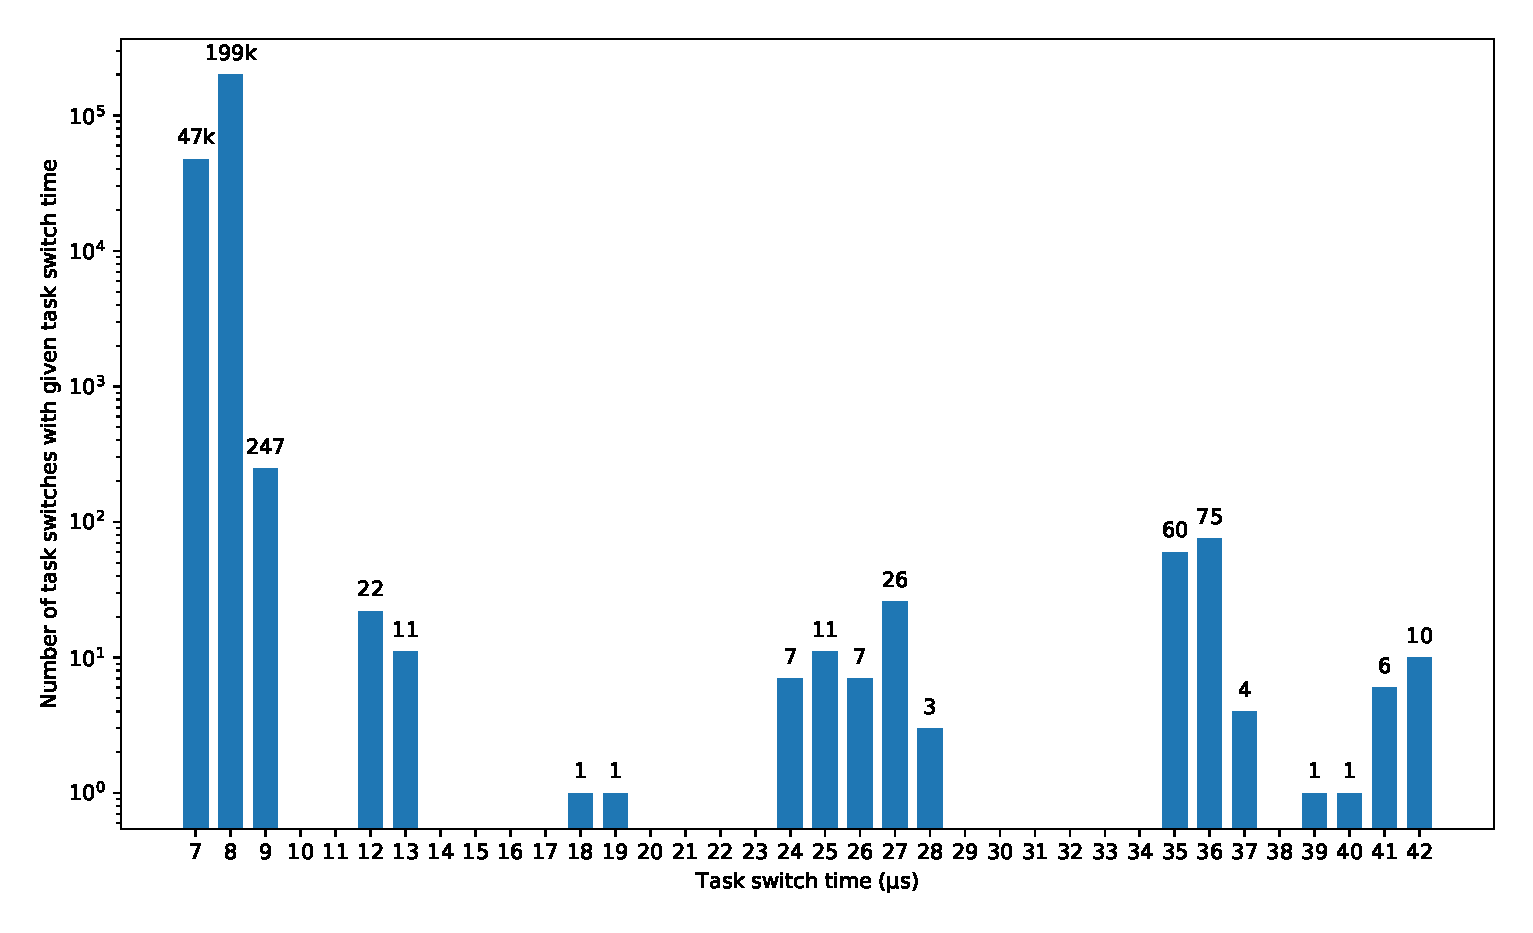
\includegraphics[width=0.8\textwidth]{task_switch_time.eps}
    \caption{A histogram of task switch time between round-robin tasks (mean 8.17µs; std. dev. 0.90µs). Total samples: 1,024,000.}
    \label{fig:rrhist}
\end{figure}

\subsection{\ucosiii scheduler: task switch time as the number of priorities increases}
As the number of priorities increases, the size of the priority bitmap increases linearly. Since we search the priority bitmap each time we perform a task switch, we would expect task switch time to increase linearly as well. In figure~\ref{fig:prioboxplot}, a set of box plots of task switch time is shown, for a varying number of priorities. For each number of priorities, 32 tasks were spaced evenly in the priority space, and the time to switch between them was measured for each task switch for a duration of five seconds. As expected, the mean task switch time increases linearly (visible as a curved line in this log-log plot due to the non-zero y-intercept). Additionally, the variance increases greatly as the number of priorities increases.

\begin{figure}[htpb]
    \centering
    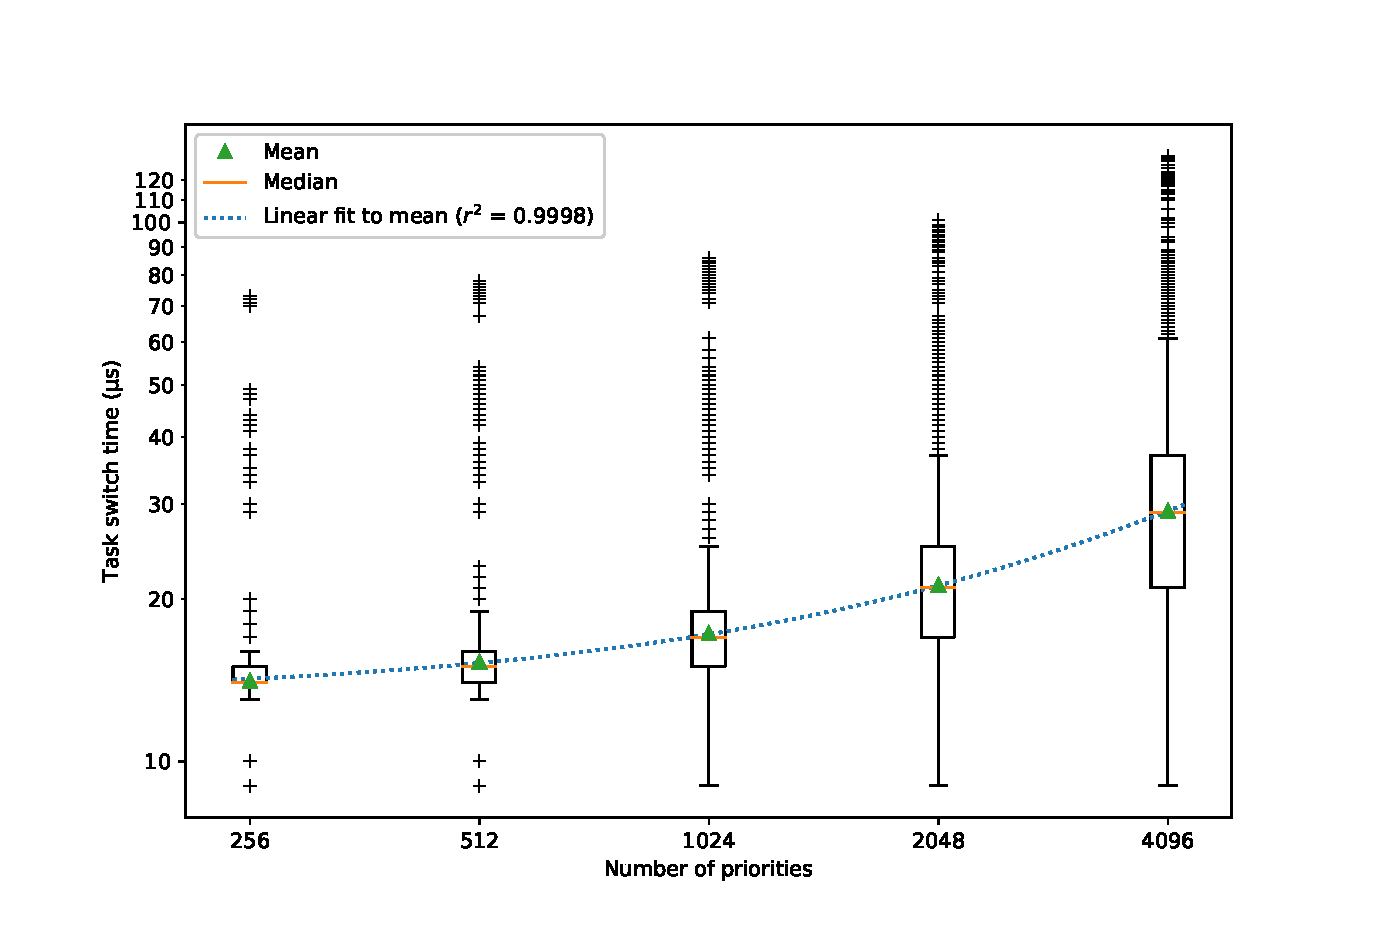
\includegraphics[width=0.8\textwidth]{boxplot.eps}
    \caption{Box plots of task switch time as the number of priorities increases. As task switches were measured over a fixed period of time, the number of samples for each box plot varies, from a minimum of 547,535 to a maximum of 938,926.}
    \label{fig:prioboxplot}
\end{figure}

\section{Task set response time and schedulability}
\subsection{Determining worst-case execution times}
As discussed in the scheduling chapter, when using guarantee-based scheduling, an accurate worst-case execution time estimation for tasks is paramount to ensure that the provided guarantees actually have meaning. The same is true when evaluating scheduling performance. However, worst-case execution time estimation is a difficult task for even simple code, and in these experiments, I would like to greatly vary task sets, requiring me to perform worst-case execution time analysis for many task sets. Therefore, I have chosen to simulate actual tasks by executing instructions which do not perform any useful work, but have very predictable timing characteristics. These timing characteristics can be found in chapter 16 of the ARM Technical Reference Manual for the Pi's ARM1176JZF-S processor\cite{arm:arm1176}.

\begin{lstlisting}
wait_for_cycles:
    subs r0, r0, #1
    bne wait_for_cycles
    bx lr
\end{lstlisting}


\begin{enumerate}
    \item The \code{wait_for_cycles} subroutine waits for $2r_0 ~10-14$ cycles. A description of the cycle count of the used instructions is as follows;
    \item Data processing instructions not targeting the program counter and without included shifts, such as this \code{subs} instruction, take a single cycle\cite[p. 16-7]{arm:arm1176}.
    \item Branch instructions such as \code{bne} have complex timing characteristics, since the ARM1176JZF-S processor includes both a static and a dynamic branch predictor, as well as a return prediction stack\cite[p. 16-2]{arm:arm1176}. Let us assume a scenario where we want to wait for a number of cycles that is greater than one.

    The first time this branch executes and when it is not in the 128-entry dynamic branch predictor cache, it will take 4 cycles, as it will be correctly predicted to be taken by the static branch predictor, which predicts that backward branches are always taken\cite[p. 5-5]{arm:arm1176}.

    After this, it will be set to be weakly taken in the dynamic branch predictor. This correct prediction allows the branch to take a single cycle\footnote{If folded out, the branch could take zero cycles. Since branch folding is hard to predict, however, my startup code disables branch folding.}\cite{arm:arm1176}.

    After the last iteration, the branch will be mispredicted, and as the subtraction instruction directly precedes the branch instruction, this incurs a cost of 6 cycles.
    \item The return instruction takes 4 or 5 cycles depending on whether the code is interrupted - if it is, the return stack will most likely be empty and therefore cause an extra cycle.
\end{enumerate}

The cycle count for the given instructions could vary based on presence in the instruction cache or other architectural buffers (such as the instruction prefetch buffer). Most important, however, is the timing of the instructions in the inner loop, as they account for the bulk of the cycles used. Experimentally, the 2-cycle inner loop behavior is verified in \code{apps/waittest/app.c}.

One issue with using cycles to wait for a given period of time is the variability of the Pi's clock speed. The Pi will, however, only throttle the clock speed in two cases; when an undervoltage is detected (this occurs when the power supply cannot supply 5 volts at the requested amperage, so the voltage drops) or when the core temperature gets above 80 degrees\cite{rpi:gpuclockpower}. Measuring the GPIO voltage during system stress reveals that my power supply can consistently supply five volts. The second case does not occur on first-generation Pis due to its low-power processor (later generations have higher clock speeds and are multi-core chips, and therefore have a larger thermal output and are at higher risk of overheating). Therefore, we can rely on the system clock staying constant.

\chapter{Discussion and conclusion}
As discussed in the introduction, using guarantee-based scheduling is yet another tool in the toolbox of achieving predictable and safe real-time computing. I hope this thesis gives a good overview of the required information needed to use guarantee-based scheduling, and shows where guarantee-based scheduling is strong.

\section{Further Research}


{
    \hfuzz=8pt
    \printbibliography
}
\end{document}
